\documentclass[11pt, a4paper, abstract=true]{scrartcl}
\usepackage[sexy]{evan}
\usepackage{float}
\usepackage[margin=1.00in]{geometry}
\usepackage{multirow}
\usepackage{longtable}
\def\arraystretch{1.20}

% \clearpairofpagestyles
\setkomafont{pagenumber}{\itshape}
\KOMAoptions{}
\ohead{\footnotesize \textbf{\leftmark}}
\ihead{\footnotesize \textsc{Lab Report I}}
\cfoot{\pagemark}
\begin{document}
\subject{
    CH1202: Lab Report
}
\title{
    \huge Determination of \\
    Isoelectric Point (pI) of Amino Acid
}
\author{
    Abhisruta Maity \\
    {\normalsize 21MS006}
    \plusemail{am21ms006@iiserkol.ac.in}
}
\date{}
\publishers{
    \normalsize \emph{Indian Institute of Science Education and Research, Kolkata \\
    Mohanpur, West Bengal, 741246, India}
}
\maketitle

\tableofcontents

\newpage

\section{Equation}

For this experiment of determination of isoelectric point of amino acid, as an amino acid, we use mainly two essential equations, namely 
\begin{proposition}[Henderson-Hasselbalch Equation]
    Suppose, \(K_a\) be the dissociation constant of acid \(\text{HA}\). A buffer solution is prepared with that acid having concentration \([\text{HA}]\) and concentration of the corresponding conjugate base in that solution is \([\text{A}^-]\). Then the pH of the buffer solution is given by 
    \begin{equation*}
        pH = pK_a + \log{\frac{[\text{A}^-]}{[\text{HA}]}}
    \end{equation*}
\end{proposition}

\begin{definition}[Isoelectric Point of an Amino Acid]
    Given an amino acid, it stays in the form of zwitterion, i.e., its neutral form. But since, the amine and the carboxyl group have different base and acid strengths, it does not necessarily stay neutral at \(pH = 7\). Hence, we define the isoelectric point \(pI\) as the \(pH\) where the amino acid becomes neutral. 
\end{definition}

\begin{proposition}[Isoelectric Point \(pI\)]
    Deciphering the definition and some mathematical calculations yield 
    \begin{equation*}
        pI = \frac{pK_{a1} + pK_{a2}}{2}
    \end{equation*}
    The \(pK_{a1}\) and \(pK_{a2}\) are respectively the acid dissociation constants for the reactions given in the figure below.

    Include figure ??
\end{proposition}

\section{Dataset}

\subsection*{Preparation of 100 mL standard 0.1 N KHP solution}
\begin{itemize}
    \item Weight taken = 2.050 g
    \item Weight to be taken = 2.04222 g
    \item Strength of KHP solution = 20.5 g/L
\end{itemize}
\subsection*{Calculation}
\texttt{Molecular weight of KHP = 204.222 g/mol \\ Strength = 2.05 g/0.1 L = 20.5 g/L}
% \usepackage{multirow}
\begin{table}[H]
\centering
\begin{tabular}{|c|c|ccc|c|c|}
\hline
\multirow{2}{*}{Sl. No.} &
  \multirow{2}{*}{\begin{tabular}[c]{@{}c@{}}Volume of\\ KHP (mL)\end{tabular}} &
  \multicolumn{3}{c|}{Burette Reading (mL)} &
  \multirow{2}{*}{\begin{tabular}[c]{@{}c@{}}Average\\ Volume (mL)\end{tabular}} &
  \multirow{2}{*}{\begin{tabular}[c]{@{}c@{}}Strength of NaOH\\ Solution (g/L)\end{tabular}} \\ \cline{3-5}
  &    & \multicolumn{1}{c|}{Initial} & \multicolumn{1}{c|}{Final} & Difference &                         &                        \\ \hline
1 & 10 & \multicolumn{1}{c|}{0}       & \multicolumn{1}{c|}{10.1}  & 10.1       & \multirow{3}{*}{10.17} & \multirow{3}{*}{3.93} \\ \cline{1-5}
2 & 10 & \multicolumn{1}{c|}{0}       & \multicolumn{1}{c|}{10.2}  & 10.2       &                         &                        \\ \cline{1-5}
3 & 10 & \multicolumn{1}{c|}{0}       & \multicolumn{1}{c|}{10.2}  & 10.2       &                         &                        \\ \hline
\end{tabular}
\caption{Standardization of NaOH solution using standard 0.1 N KHP solution}
\end{table}

\subsection*{Calculation}

\texttt{Molecular weight of NaOH = 40 g/mol} \[\mathtt{N_1 V_1 = N_2 V_2}\] \texttt{where,} \(\mathtt{N_1 = 20.5 \; g/L; V_1 = 10}\) \texttt{mL}; \(\mathtt{V_2 = 10.17}\) \texttt{mL}. \texttt{Hence,} \[\mathtt{N_2 \approx 3.93 \; g/L}\]


{\centering
    \begin{longtable}{|l|l|l|l|l|}
    \hline
    \(V\)      & \(pH\)      &   \(\Delta V\)   & \(\Delta pH\)     &  \(\Delta pH / \Delta V\)    \\ \hline
    0     & 1.41  & 0.5  & 0.03 & 0.06 \\ \hline
    0.5   & 1.44  & 0.5  & 0.04 & 0.08 \\ \hline
    1     & 1.48  & 0.5  & 0.05 & 0.1  \\ \hline
    1.5   & 1.53  & 0.5  & 0.05 & 0.1  \\ \hline
    2     & 1.58  & 0.5  & 0.06 & 0.12 \\ \hline
    2.5   & 1.64  & 0.5  & 0.06 & 0.12 \\ \hline
    3     & 1.7   & 0.5  & 0.05 & 0.1  \\ \hline
    3.5   & 1.75  & 0.5  & 0.07 & 0.14 \\ \hline
    4     & 1.82  & 0.5  & 0.07 & 0.14 \\ \hline
    4.5   & 1.89  & 0.5  & 0.06 & 0.12 \\ \hline
    5     & 1.95  & 0.5  & 0.08 & 0.16 \\ \hline
    5.5   & 2.03  & 0.5  & 0.09 & 0.18 \\ \hline
    6     & 2.12  & 0.5  & 0.09 & 0.18 \\ \hline
    6.5   & 2.21  & 0.5  & 0.1  & 0.2  \\ \hline
    7     & 2.31  & 0.5  & 0.11 & 0.22 \\ \hline
    7.5   & 2.42  & 0.5  & 0.15 & 0.3  \\ \hline
    8     & 2.57  & 0.2  & 0.08 & 0.4  \\ \hline
    8.2   & 2.65  & 0.2  & 0.07 & 0.35 \\ \hline
    8.4   & 2.72  & 0.2  & 0.08 & 0.4  \\ \hline
    8.6   & 2.8   & 0.2  & 0.09 & 0.45 \\ \hline
    8.8   & 2.89  & 0.2  & 0.09 & 0.45 \\ \hline
    9     & 2.98  & 0.2  & 0.16 & 0.8  \\ \hline
    9.2   & 3.14  & 0.2  & 0.13 & 0.65 \\ \hline
    9.4   & 3.27  & 0.1  & 0.11 & 1.1  \\ \hline
    9.5   & 3.38  & 0.2  & 0.33 & 1.65 \\ \hline
    9.7   & 3.71  & 0.1  & 0.12 & 1.2  \\ \hline
    9.8   & 3.83  & 0.05 & 0.17 & 3.4  \\ \hline
    9.85  & 4     & 0.05 & 0.27 & 5.4  \\ \hline
    9.9   & 4.27  & 0.05 & 0.53 & 10.6 \\ \hline
    9.95  & 4.8   & 0.05 & 1.19 & 23.8 \\ \hline
    10    & 5.99  & 0.05 & 1.01 & 20.2 \\ \hline
    10.05 & 7     & 0.05 & 0.44 & 8.8  \\ \hline
    10.1  & 7.44  & 0.05 & 0.24 & 4.8  \\ \hline
    10.15 & 7.68  & 0.05 & 0.18 & 3.6  \\ \hline
    10.2  & 7.86  & 0.05 & 0.12 & 2.4  \\ \hline
    10.25 & 7.98  & 0.05 & 0.1  & 2    \\ \hline
    10.3  & 8.08  & 0.1  & 0.16 & 1.6  \\ \hline
    10.4  & 8.24  & 0.1  & 0.13 & 1.3  \\ \hline
    10.5  & 8.37  & 0.1  & 0.09 & 0.9  \\ \hline
    10.6  & 8.46  & 0.2  & 0.16 & 0.8  \\ \hline
    10.8  & 8.62  & 0.2  & 0.17 & 0.85 \\ \hline
    11    & 8.79  & 0.3  & 0.16 & 0.53 \\ \hline
    11.3  & 8.95  & 0.5  & 0.12 & 0.24 \\ \hline
    11.8  & 9.07  & 0.2  & 0.07 & 0.35 \\ \hline
    12    & 9.14  & 0.5  & 0.14 & 0.28 \\ \hline
    12.5  & 9.28  & 0.5  & 0.11 & 0.22 \\ \hline
    13    & 9.39  & 0.5  & 0.11 & 0.22 \\ \hline
    13.5  & 9.5   & 0.5  & 0.1  & 0.2  \\ \hline
    14    & 9.6   & 0.5  & 0.1  & 0.2  \\ \hline
    14.5  & 9.7   & 0.5  & 0.09 & 0.18 \\ \hline
    15    & 9.79  & 0.5  & 0.09 & 0.18 \\ \hline
    15.5  & 9.88  & 0.5  & 0.12 & 0.24 \\ \hline
    16    & 10    & 0.5  & 0.09 & 0.18 \\ \hline
    16.5  & 10.09 & 1    & 0.16 & 0.16 \\ \hline
    17.5  & 10.25 & 1    & 0.14 & 0.14 \\ \hline
    18.5  & 10.39 & 0.5  & 0.13 & 0.26 \\ \hline
    19    & 10.52 & 0.5  & 0.15 & 0.3  \\ \hline
    19.5  & 10.67 & 0.5  & 0.2  & 0.4  \\ \hline
    20    & 10.87 & 0.2  & 0.08 & 0.4  \\ \hline
    20.2  & 10.95 & 0.2  & 0.08 & 0.4  \\ \hline
    20.4  & 11.03 & 0.1  & 0.04 & 0.4  \\ \hline
    20.5  & 11.07 & 0.1  & 0.04 & 0.4  \\ \hline
    20.6  & 11.11 & 0.1  & 0.04 & 0.4  \\ \hline
    20.7  & 11.15 & 0.2  & 0.08 & 0.4  \\ \hline
    20.9  & 11.23 & 0.2  & 0.08 & 0.4  \\ \hline
    21.1  & 11.31 & 0.2  & 0.07 & 0.35 \\ \hline
    21.3  & 11.38 & 0.2  & 0.06 & 0.3  \\ \hline
    21.5  & 11.44 & 0.5  & 0.15 & 0.3  \\ \hline
    22    & 11.59 & 0.5  & 0.11 & 0.22 \\ \hline
    22.5  & 11.7  & 0.5  & 0.09 & 0.18 \\ \hline
    23    & 11.79 & 0.5  & 0.07 & 0.14 \\ \hline
    23.5  & 11.86 & 0.5  & 0.1  & 0.2  \\ \hline
    24    & 11.96 & 0.5  & 0.04 & 0.08 \\ \hline
    24.5  & 12    & 0.5  & 0.06 & 0.12 \\ \hline
    25    & 12.06 &      &      &      \\ \hline
    \caption{Titration of amino acid using NaOH solution}
    \end{longtable}
}

\section{Plots}

\begin{figure}[H]
    \centering
    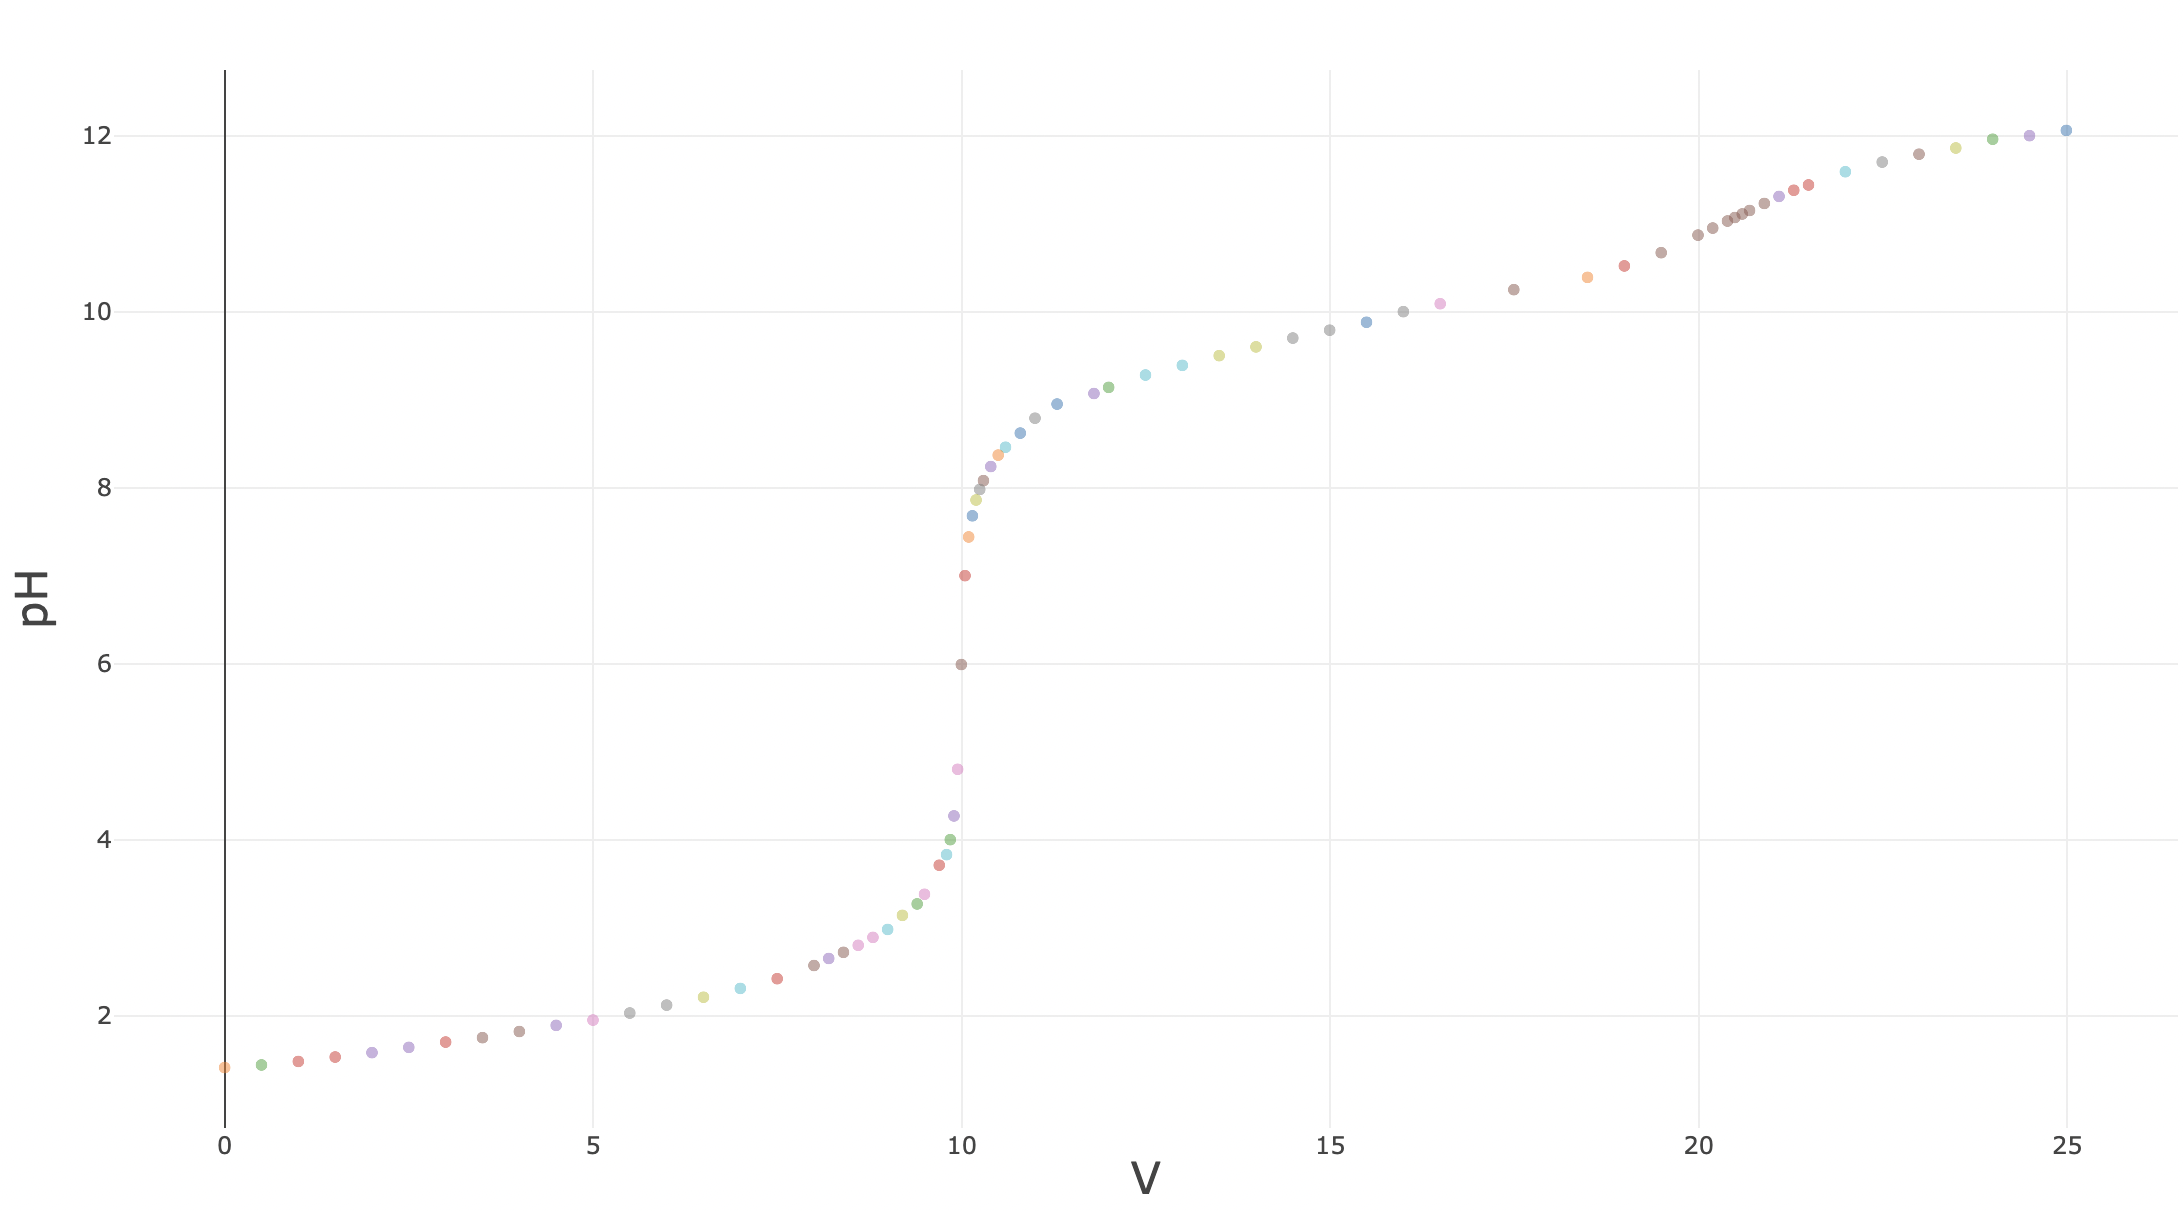
\includegraphics[scale=0.4]{data2.png}
    \caption{\(pH\) vs. \(V\)}
\end{figure}

\begin{figure}[H]
    \centering
    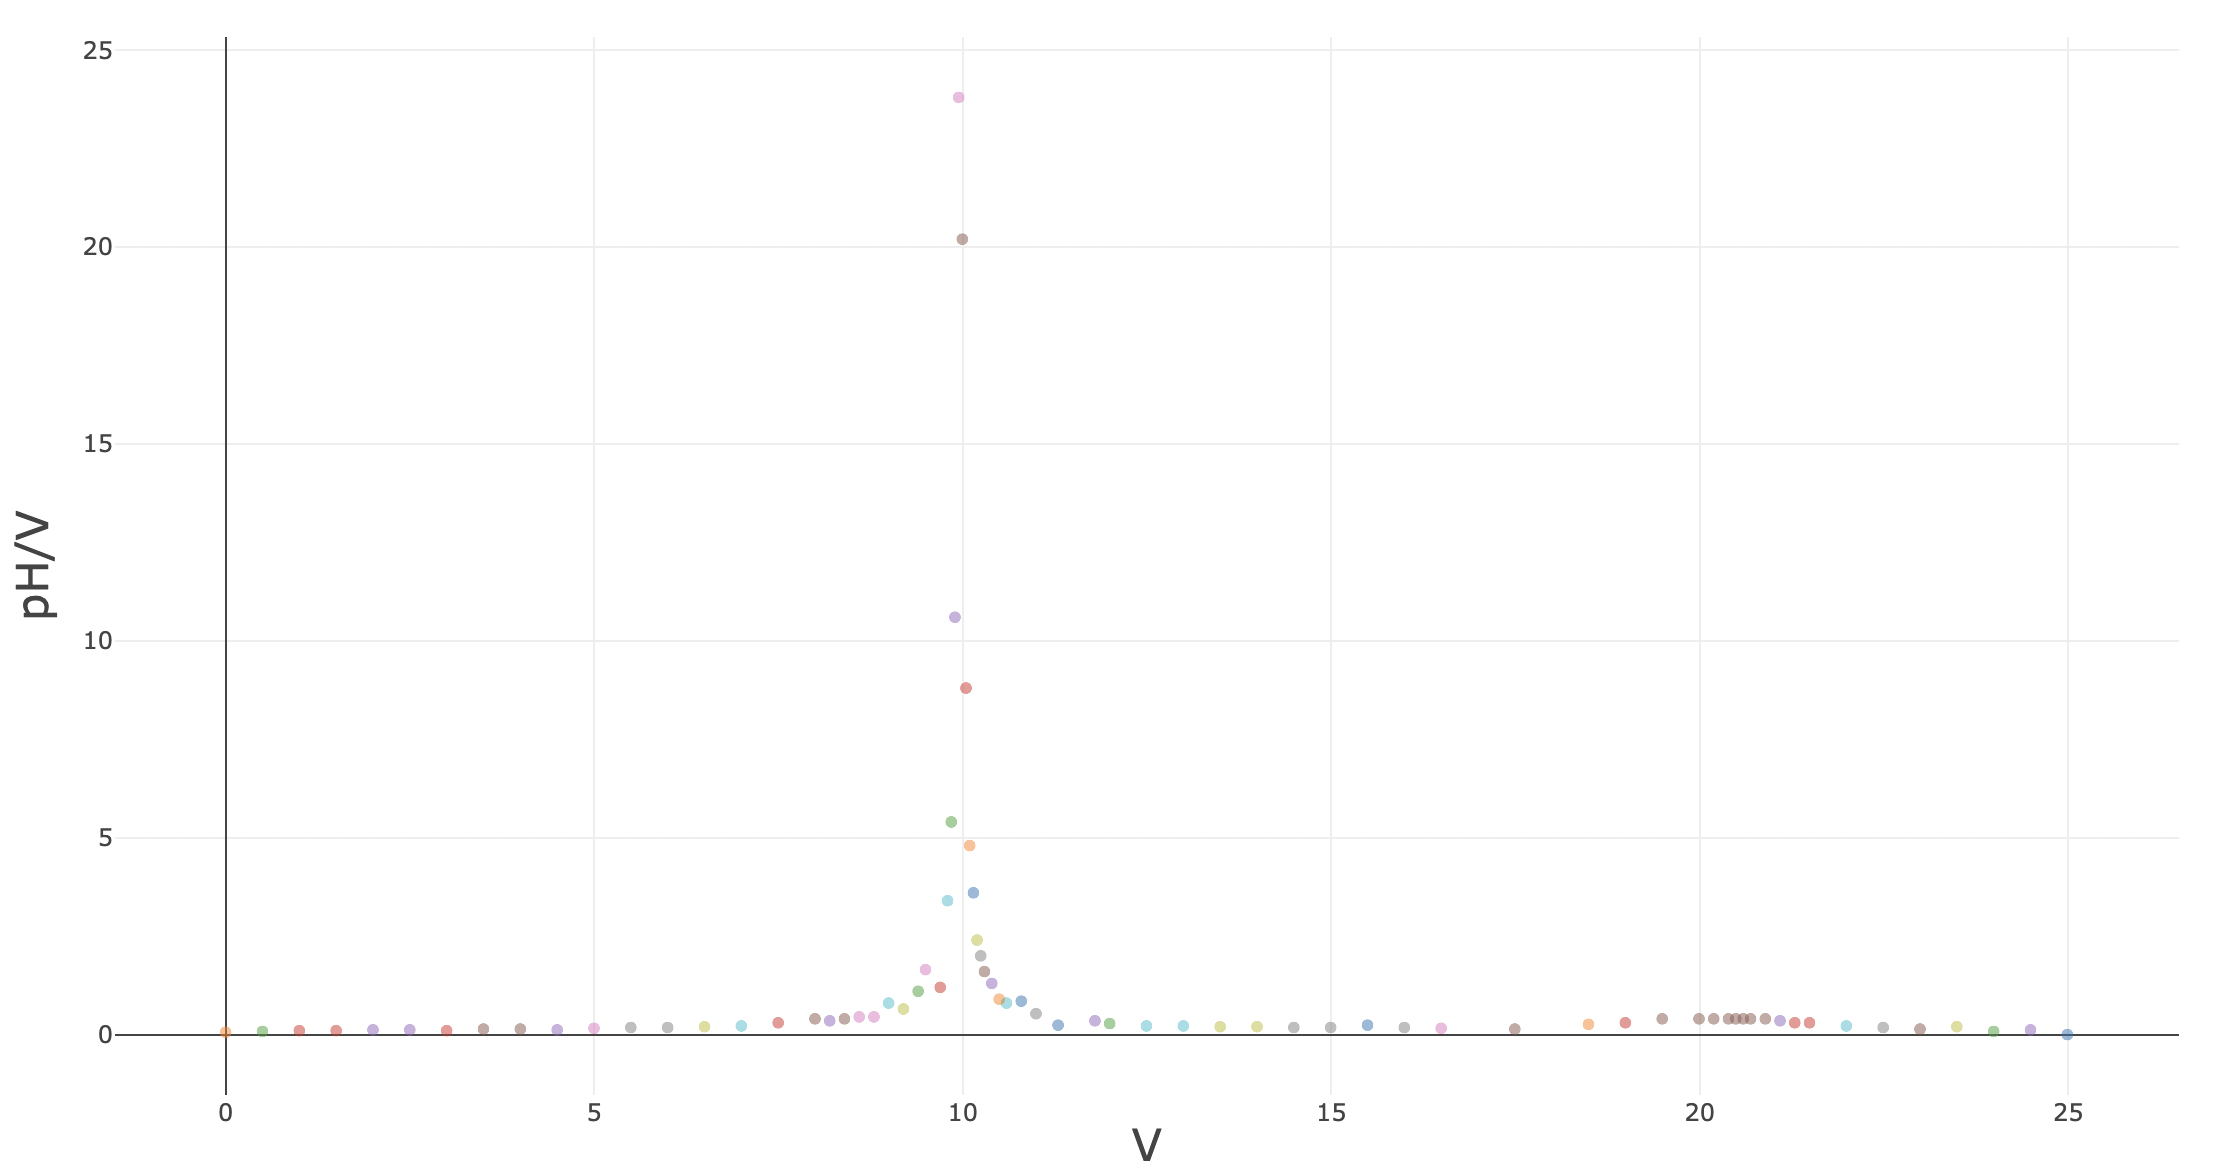
\includegraphics[scale=0.4]{data.png}
    \caption{\(\Delta pH/\Delta V\) vs. \(V\)}
\end{figure}

\textbf{Please Turn Over.}

\section{Results}

First equivalence point = 9.95 mL (The big peak). So, half the volume at first equivalence point would give \(pK_{a1} \approx 1.95\) at volume \(9.95/2 = 4.975\) mL. And, second equivalence point = 20.4 mL (The tiny peak). So, half the volume from the first peak to second peak is \(20.4 - 9.95/2 = 5.225\) mL. Hence, the \(pK_{a2} \approx 9.79\) at volume  \(9.95 + 5.225 = 15.175\) mL. Therefore, we found the isoelectric point \[pI = \frac{1.95 + 9.79}{2} = \boxed{5.87}\]

\section{Acknowledgements}

\textsc{Thanks} to our instructors for exposing to this nice experiment.






\end{document}